\newpage
\subsection{Atomic Design Systems} \label{Atomic Design Systems}
% NOTE: Add pictures of atoms, ... in use
So, let us take a closer look at Atomic Design and the reason why I believe it is the best fitting
design system methology for Design and Code collaboration. Let's begin by looking at how the web
designer Brad Frost used chemistry to define a hierarchical system. \\\\
\textbf{Atoms} \\
Atoms are the smallest building blocks of the design. They are the basic elements like buttons,
textfields, colors, fonts or icons. Things that cannot be broken down any further. \\\\
\textbf{Molecules} \\
Molecules are groups of atoms that together form a simple group of UI. For example, combining
a headline, an icon and filter buttons it would form a neat filter bar. \\\\
\textbf{Organisms} \\
Organisms are more complex groups of UI elements. They can be a combination of atoms, molecules and
also other organisms. When combining the filter bar molecule, a few buttons and a blog post grid
organism, it would form a functional blog post overview organism. \\\\
\textbf{Templates} \\
Templates are like blueprints of pages. They consist of organisms and molecules and define the
layout of a page, giving actual meaning to the UI elements. \\\\
\textbf{Pages}\\
Pages take templates as a basis and fill them with actual content. These represent how the final
delivered product will or should look like. \\
\vglcite[43,53]{frostAtomicDesign2016}\\

Picturing this methodology as building with Lego often helps improve understanding. Atoms can be
seen as individual Lego bricks which cannot be made any smaller. These bricks can be stacked
together creating bigger more complex builds. By using these defined pieces, a Lego world can be
construced that always looks consistent, but is still flexible enough to build anything.

While this analogy seems simple, it is actually quite powerful, since it demonstrates exactly what
we want from design systems. Having a set of clearly defined rules, which give both designers and
engineers the time to actually focus on solving user needs without concerns about the design
getting inconsistent or feeling too constrained. \vglcite[13]{vesselovBuildingDesignSystems2019}

\subsubsection{Advantages and Drawbacks}
Having such a hierarchical component based design system has major advantages but also comes with
drawbacks. If we know what to look out for, we can be prepared to tackle these challenges. \\\\
\begin{itemize}
	\item Advantages
	      \begin{description}
		      \item[Support iterative workflows] - Working with Atomic Design supports an iterative
		            workflow. You can start with the smallest elements, build up some definitions and then
		            take a step back to look at how they work together. As soon as you notice that
		            something is not working together, you can go back and adjust the smaller
		            elements. Having this flexibility, while still having a clear structure, working
		            iteratively becomes much easier. \vglcite[57]{frostAtomicDesign2016}
		      \item[Changing it once, changes it everywhere] - Let's say you notice that the padding
		            of a button is too small. You can change it in the button definition and all buttons
		            accross the whole design system using this definition will be updated. This way,
		            you never have to completely redo everything, since there is always one source
		            of truth.
		      \item[Opportunity to work as close with devs as possible] - As already mentioned
		            before, the structure of the system is very close to how devs actually work.
		            If you think about it, integrating this hierarchical, component-based system
		            into the design process from the start should naturally streamline collaboration
		            and make the handoff between design and development much smoother.

		            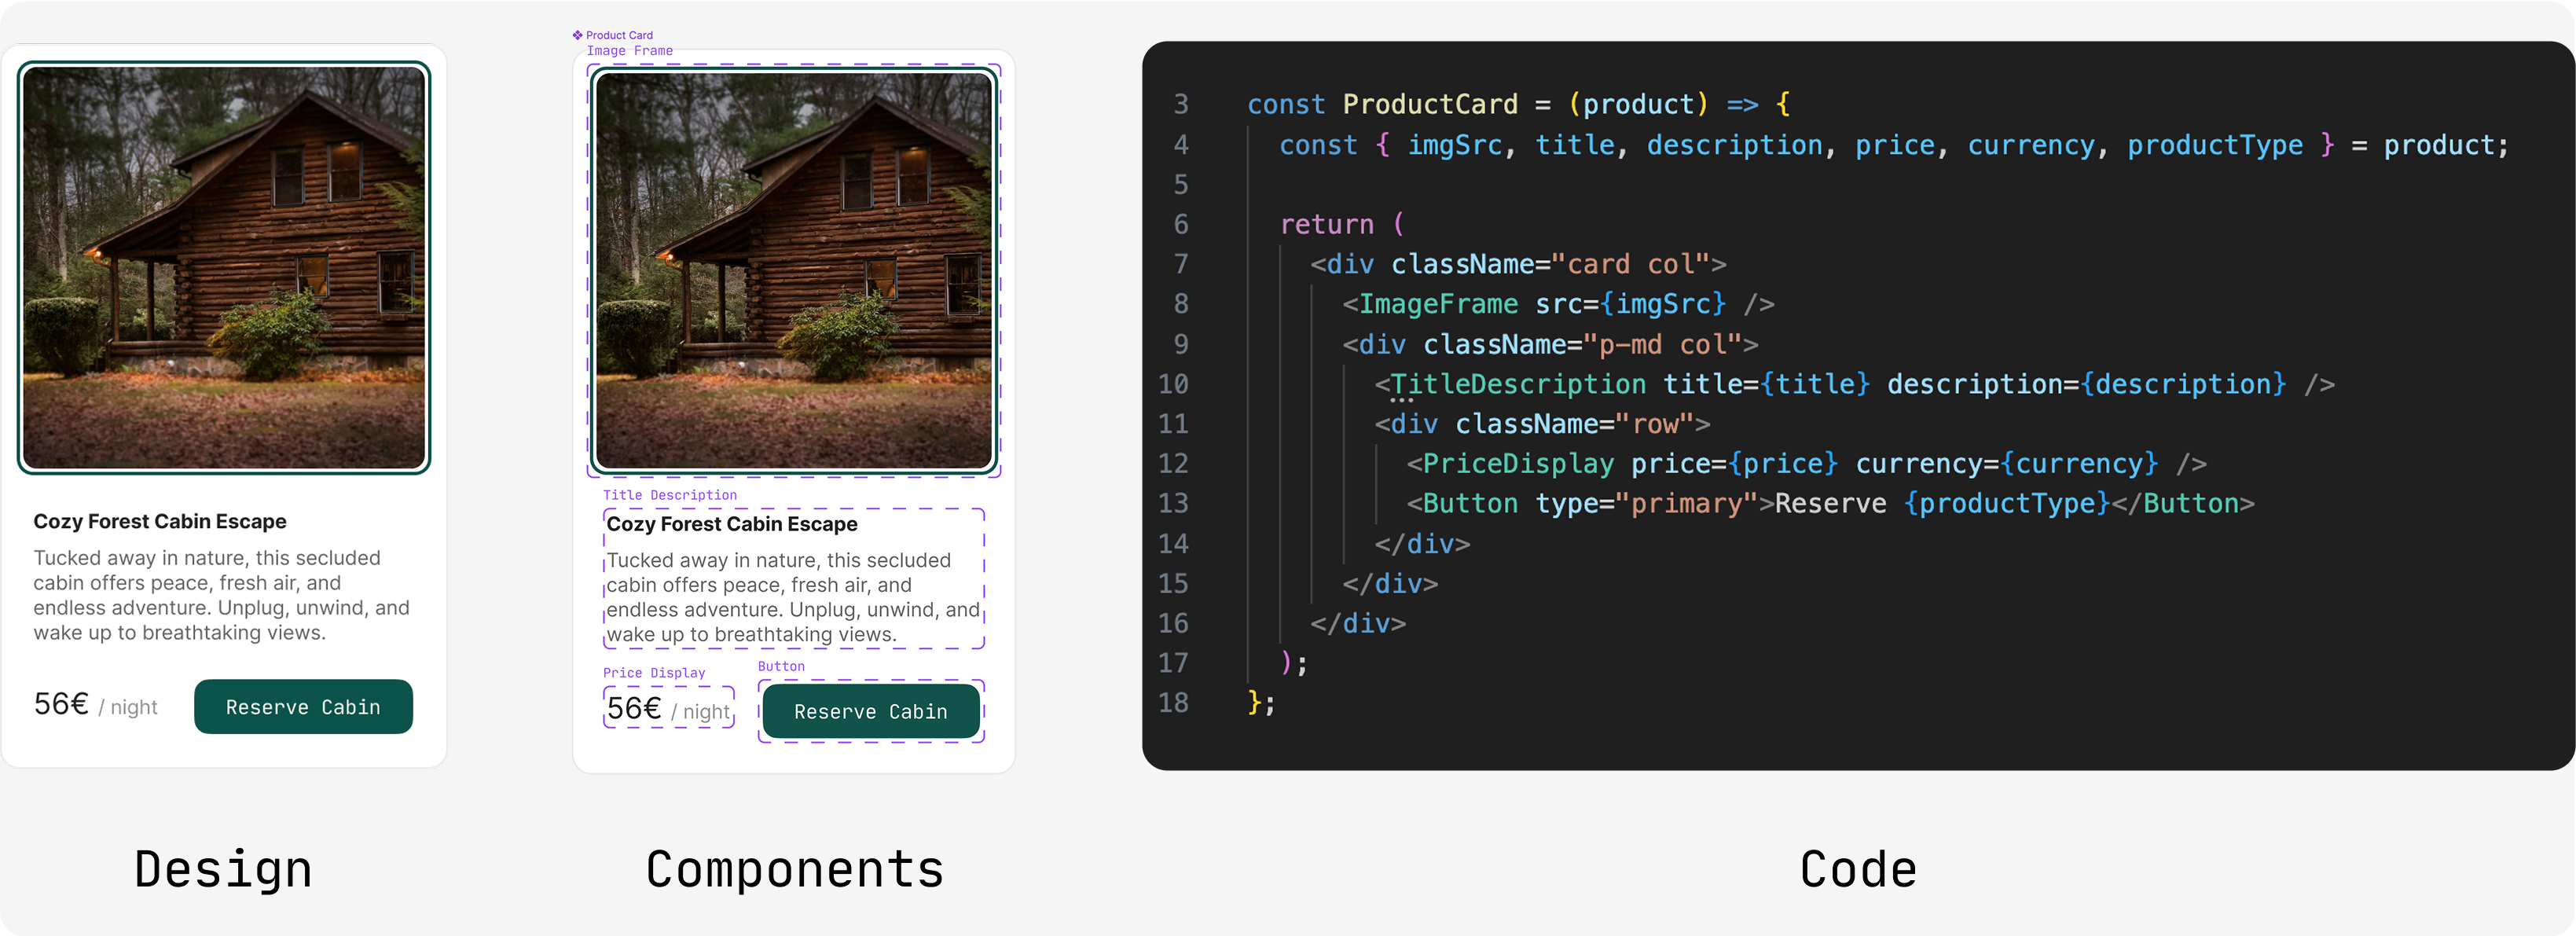
\includegraphics[width=400pt, height=\textheight,keepaspectratio]{2_chapter/Design To Code Similarities.jpg}
					^^ Sample image showing how similar the design and code can be in terms of structure
		            % NOTE: Show Picture UI Design and Developed Code and how similar it can be
	      \end{description}
	\item Drawbacks
	      \begin{description}
		      \item[Confusion about nomenclature] - Many teams struggle with the abstract terms of
		            Atomic Design and have a hard time assigning components to the right category. The
		            team at Bridge Studio for example, decided to use different terms like "Foundations"
		            or "Components" to make it easier to group and understand the elements. However, they
		            still kept the mindset of Atomic Design.
		            (https://www.linkedin.com/pulse/whats-wrong-atomic-design-james-eccleston)

		            Brad Frost actually encourages teams to adapt
		            the system to their needs, but keeping the core principles in mind. \vglcite[59]{frostAtomicDesign2016}
		            % https://www.linkedin.com/pulse/whats-wrong-atomic-design-james-eccleston it has to
		            % be altered a little bit to fit needs or Sarah Vesselov's book page 28
		      \item[Feeling too restricted] - 
	      \end{description}
\end{itemize}
 
\subsubsection{Common Best Practices}
% Basically say that naming should be clear but not too specific, Using Figma features for design tokens such as variables and styles. Not overdoing it right
% from the start cite: Sarah Vesselov's book page 21
% Think of it as a process iteratively evolving over time like the product it is used for. The Design
% System is never a finished product.
% https://uxdesign.cc/to-create-an-excellent-design-system-treat-it-like-a-collaborative-process-6602376bfef6
